\documentclass[letterpaper,11pt,notitlepage,fleqn]{article}

%\usepackage{nopageno} %gets rid of page numbers
\usepackage{alltt}                                           
\usepackage{float}
\usepackage{color}
\usepackage{indentfirst}
\usepackage{url}
\usepackage{balance}
\usepackage[TABBOTCAP, tight]{subfigure}
\usepackage{enumitem}
\usepackage{pstricks, pst-node}
\usepackage{geometry}
\geometry{textheight=9in, textwidth=6.5in} %sets 1" margins 
\newcommand{\cred}[1]{{\color{red}#1}} %command to change font to red
\newcommand{\cblue}[1]{{\color{blue}#1}} % ...blue
\usepackage{hyperref}
\usepackage{textcomp}
\usepackage{listings}
\usepackage{graphicx}
\usepackage{amsfonts}
\usepackage{amsmath}

% Code snippets color
\definecolor{dkgreen}{rgb}{0,0.6,0}
\definecolor{gray}{rgb}{0.5,0.5,0.5}
\definecolor{mauve}{rgb}{0.58,0,0.82}
\lstset{frame=tb,
  language=C,
  aboveskip=3mm,
  belowskip=3mm,
  showstringspaces=false,
  columns=flexible,
  basicstyle={\small\ttfamily},
  numbers=none,
  numberstyle=\tiny\color{gray},
  keywordstyle=\color{blue},
  commentstyle=\color{dkgreen},
  stringstyle=\color{mauve},
  breaklines=true,
  breakatwhitespace=true,
  tabsize=3
}
\lstdefinelanguage{diff}{
  morecomment=[f][\color{blue}]{@@},     % group identifier
  morecomment=[f][\color{red}]-,         % deleted lines 
  morecomment=[f][\color{green}]+,       % added lines
  morecomment=[f][\color{magenta}]{---}, % Diff header lines (must appear after +,-)
  morecomment=[f][\color{magenta}]{+++},
}
% End color
\def\name{Sam Quinn}

\parindent = 0.4444 in
\parskip = 0.2 in

\begin{document}
\begin{titlepage}
\vspace*{\fill}

\newcommand{\HRule}{\rule{\linewidth}{0.5mm}} % Defines a new command for the horizontal lines, change thickness here

\center % Center everything on the page

%----------------------------------------------------------------------------------------
%TITLE SECTION
%----------------------------------------------------------------------------------------

%\includegraphics[scale=.5]{image.eps}
\HRule \\[0.4cm]
{ \huge \bfseries Homework \#1}\\[0.4cm] % Title of your document

%----------------------------------------------------------------------------------------
%HEADING SECTIONS
%----------------------------------------------------------------------------------------

\textsc{\LARGE Oregon State University}\\[0.5cm] % Name of your university/college
\textsc{\Large ECE 478 Network Security}\\[0.5cm] % Major heading such as course name
\textsc{\large Spring 2016}\\[0.5cm] % Minor heading such as course title


\HRule \\[1.5cm]
%----------------------------------------------------------------------------------------
%AUTHOR SECTION
%------------------------------------ ----------------------------------------------------

\begin{minipage}{0.4\textwidth}
\begin{flushleft} \large
\emph{Student:}\\
        \noindent \textbf{Sam \textsc{Quinn}} \\ % Your name
        {\small Quinnsa@Oregonstate.edu}
        \end{flushleft}
        \end{minipage}
        ~
        \begin{minipage}{0.4\textwidth}
        \begin{flushright} \large
        \emph{Professor:} \\
            \noindent \textbf{Dr. Attila A \textsc{Yavuz}} \\ % Supervisor's Name
            {\small Attila.Yavuz@oregonstate.edu}
            \end{flushright}
            \end{minipage}\\[3cm]

                %----------------------------------------------------------------------------------------
                %DATE SECTION
                %-----------------    -----------------------------------------------------------------------

{\large \today}\\[3cm] % Date, change the \today to a set date if you want to be precise

%----------------------------------------------------------------------------------------
%LOGO SECTION
%------   ----------------------------------------------------------------------------------

    
\includegraphics[scale=0.5]{coe.eps}\\[1cm] % Include a department/university logo - this will require the graphicx package

%----------------------------------------------------------------------------------------

\vfill % Fill the rest of the page with whitespace



\end{titlepage}

\tableofcontents
\newpage

\section{Question about basic concepts:}
\noindent \textbf{What are the main security/performance trade-offs for symmetric and asymmetric cryptography to be deployed in practice? Could you give real-life scenarios where symmetric and asymmetric crypto could be more suitable?}

Symmetric and asymmetric cryptography are the two basic forms of encryption with each functioning differently than one another. Symmetric cryptography is faster but needs the secret key share between all parties before hand. Since there is one secret key that is shared between all parties before hand it all encryption as well as decryption is done with the same key, meaning that all parties use the same key. Symmetric is better when dealing with only trusted parties since you cannot
establish authentication with only one secret key. Symmetric encryption is ideal for encrypting personal files where the secret key would not need to be shared.\\
\indent Asymmetric cryptography dose not need the secret key to be shared before hand. Asymmetric encryption needs two keys, a private key and a public key. The public key may be shared with the presence of an eavesdropper with no security penalties. Asymmetric encryption keys do not need to be pre-shared with parties, and since every party has their own key pair it will also provide authentication. Asymmetric cryptography is ideal for applications where both parties have never spoken before, for example SSH. 

\noindent \textbf{OTPs are highly secure, but why we do not see them much in practice?}


One time pad is one of the highest security since each bit of the plaintext is randomized, the random pattern used to in the OTP can only be used once or information can be extracted form the cipher text. The main problem with OTP is that the size of the key must be the size of the data, and a new key must be generated every message. 

\noindent \textbf{Does Kerckhoffs's principle contradict with the ``secret algorithm'' practice in military systems? Given sufficient financial capability, how could you incorporate Kerckhoffs's principle into such high-end systems?}

The security systems used in the military are often classified until they come up with a new method in which the old systems are released to the public. Withholding the current system from the public introduces the property of security through obscurity since the adversary does not know the algorithms used. One way to introduce Kerckhoffs's principle in to military systems would be to hire a team of skilled cryptographers to study the security systems used thus giving them complete knowledge
of the system minus the key. If the team are able to break the system then the only thing that is keeping the military security system secure is the obscurity which is very weak. However if the team is unable to break the system knowing everything but the key then the system is secure plus the added bonus of being obscure.

\section{Data Encryption Standard (DES). DES has weak keys.}
\noindent \textbf{What is the difference between a weak key, a semi-weak key and a possible weak key?}

The origin of weak, semi-weak, and possibly weak keys in DES start with how DES extracts each rounds encryption keys from the master 56bit key. The 56bit key is divided into 16 sub keys one for each cycle of the DES encryption. A weak key would be $\lbrace0\rbrace^{56}$ or $\lbrace1\rbrace^{56}$ where all of the bits are the same thus making the rotating of the keys for each cycle useless. A semi-weak key would be a key that would reverse the cycle that took place in the previous cycle. A
key that repeats with a period of 2 meaning that the rotation of keys produces exactly two keys that will be each be used 8 times. Possibly weak keys are keys that repeat with a period of 4, outputting 4 unique keys that will all be used 4 times each. (http://search.proquest.com/openview/6cc5dfe1f7c352582f2b62aa741b47dd/1?pq-origsite=gscholar) 

\noindent \textbf{What is double DES?  What kind of attack on double DES makes it useless?}

Double DES does two rounds of DES encryption with two different keys, thus making the key 112 bits long. With a meet in the middle attack the added benefit of encrypting twice does not increase the security much. 
Meet in the middle attack. The effective security gain from the single DES $2^{56}$ is increased by one exponential to $2^{57}$ in double DES. Double DES is useless because an adversary could brute force the first round (single DES) and then just pass the output to the second round without the need for any brute forcing. (http://stephanemoore.com/pdf/meetinthemiddle.pdf)

\noindent \textbf{What is triple DES?  How many keys are use in triple DES process?}

Triple DES uses three rounds of DES making the maximum security 168 bits. Triple DES can either use 2 or 3 keys, however the effective security due to the meet in the middle attack explained above is $2^{112}$. 



\section{Block Cipher Design Principles and AES}
\noindent \textbf{What is the basic design  technique,  which  is  frequently  used  to  construct  modern symmetric ciphers?}

Symmetric cryptography will use techniques to obscure the data with confusion and diffusion. Confusion is mainly accomplished by substitutions, replacing original data with new data. Diffusion is mainly accomplished by permutations, where one bit changes will permute on to all the ciphertext data to further scramble the original input. Modern symmetric ciphers will alternate substitutions and permutations.

\noindent \textbf{What are the main security properties achieved via this designed technique?}

Confusion in a symmetric cipher will help prevent attacks linear attacks. Because the data is passed through a non-linear table often created by the secret key the data is translated in a non-linear way.\\
\indent Diffusion will help prevent against pattern analysis attacks. Since every language has traceable patterns in grammar, diffusion makes these patterns much harder to spot. If one bit is changed the entire ciphertext will be changed not just the corresponding bit within the ciphertext. 

\noindent \textbf{Given the  example  of  AES,  which  functional  steps  enable achieving  these  properties?  Please provide  specific  names  of  these operations  and  briefly  explain  how  they  are  applied  in AES (all answers are brief for this question)?}

\noindent$\bullet$ Confusion: S-Box - Rijndael S-Box is a lookup matrix generated by determining the multiplicative inverse of each byte from the original input. \\
$\bullet$ Diffusion: MixColumn - AES uses a MixColumn function on the Rijndael matrix that permutes any change with data through the use of XORs. 

\noindent \textbf{What are the benefits of the use of finite field arithmetic in AES?}

Finite field arithmetic in AES is an redefinition of how to perform algebraic operations including multiplication, addition, subtraction, and division. A finite field has a finite number of integers that  

\section{Symmetric Encryption Modes}
\noindent \textbf{We have discussed various Symmetric Encryption Modes. Each of  these modes  satisfies certain properties, which can be  an  advantage or disadvantage  for  a given  application. Construct a  table providing a  summary  information  about  each mode and  its corresponding properties. For example,  each  row  of  the  table  will  be  properties  (e.g.,  parallel  operation,  ciphertext manipulation,  pre-computation,  etc.,  please  see  course  notes  for  more  properties)  and  columns are  Modes  (e.g.,  CBC,  CTR…).  Each  cell  will  take  a  value  such  as  “Yes”,  “No”,  “partially”, “high”, “low” etc. according to given encryption mode and property.}

\section{Ciphertext  manipulability}
\noindent \textbf{“Ciphertext  manipulability”  is  generally  considered  as  an  undesirable  property  for Encryption  Modes.  However,  for  modes  that  operates  in  stream  cipher  fashion  (discussed  in class), by design, it is possible to flip bits in plaintext by flipping bits of ciphertext.}
\noindent \textbf{Why is this possible?}
\noindent \textbf{Is  there  a  way  to  turn  this  (potentially)  undesirable  property  into  an  advantage, describe how if there is one?}
\noindent \textbf{Which  extra  cryptographic  function  (a  group  of  functions  discussed  in  the  class)  can be applied to the ciphertext so that the aforementioned advantage can be obtained without compromising the security?}

\noindent Hints:  (i) Consider  noisy  communication  channels  as  application  domain  to  exploit  this  feature. 
(ii) The extra cryptographic function will require annexing a small-constant tag to the ciphertext. 

\section{Encryption and Compression}
\noindent \textbf{Encryption (E) and Compression (C) are generally used together to achieve confidentiality and  efficiency  simultaneously. Given  a message M, with which order  function E  and C must be applied? What are the reasons behind of this particular order?}

\section{Symmetric key Authentication}
\noindent \textbf{In  symmetric  key  cryptography,  it  is  desirable  to  achieve  both  confidentiality  and authentication  (also  provides  integrity)  of  the  data.  These  properties  can  be  achieved  via Encryption (E) and Authentication Functions (A), respectively. What is the correct order of these operations? Lets assume the specific notation and order of these operations are as follows:} 
\begin{itemize}
    \item \textbf{Authenticate-then-Encrypt (AtE)}
    \item \textbf{Encrypt-then-Authenticate (EtA)}
    \item \textbf{Encryption and Authentication (E\&A) or the opposite way as (A\&E)}
\end{itemize}

\noindent \textbf{Discuss the security implications of these choices, which one is recommended and why?}

\noindent \textbf{Mention important crypto papers (at least one, cite it), in which the security of an important real-life  protocol  (Hint:  the  protocol  that  securely  connects  your  VPN  for  each  e-commerce transaction!)  analyzed  based  on  the  above  orders.  Explain  why  this  order  matters  a  lot  in practice?  You  may  provide  some  discussions  from  these  papers  (please  be  brief,  just  hit  on important points).}

\section{Cryptographic  hash  functions}
\noindent \textbf{Given  a modern  cryptographic  hash  function  (e.g.,  SHA) with m-bit  length  output, what is  the maximum  security  it  can  provide  in  terms  of  m  (lets  call  it  x-bit  security)? A  generalized proof  for  any  given  m-bit  hash  function  is  available  to  show  why  it  can  achieve  at  best  x-bit security.  Please  describe  this  generalized  proof  (related  birthday  attack  concept)  that  simply connects m-bit to x-bit.}

\section{Length extension}
\noindent \textbf{What  is  the  hash  length  extension  attack?  Please  describe  by  giving  some  specific  real-life examples.}

A length extension attack is an attack on HMACs with messages of varining length where an adversary may append new data to the authenticated message with the same signature. 
\begin{center}
    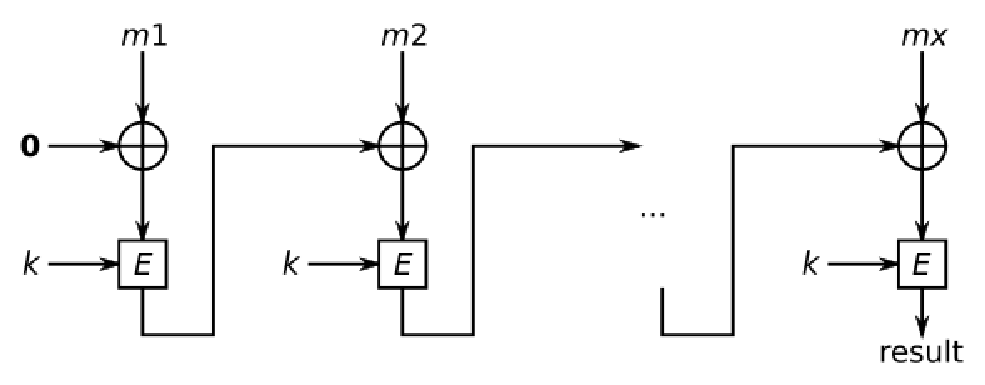
\includegraphics{cbcmac.eps}\\[1cm] % Include a department/university logo - this will require the graphicx package
\end{center}
\indent CBC-MAC is suseptible to a lenghth extention attack when the messages are not restricted to a single length. CBC-MAC will take the input message and compute the CBC encryption of the message. With the idea of a MAC to shorten the input to a fixed size, CBC-MAC will only export the last block of the message into its signature. As described above the output from $e$ will be $\otimes$ by $mx$ until the last block. An adversary is able to attack this MAC if they take the $result$ form
the original MAC $m$ and $\otimes m_{1}'$ with the $result$. This would make the $result$ cancel out the $result \otimes$ that was in $m_{1}'$. After we break the $result$ with $m_{1}'$ we are able to append anything with in $m'$ to the end of $m$ with the same signature.
\begin{center}
    $CBC\_MAC(k,m_{1},..., m_{l}) \rightarrow (m,t)$ \\ $CBC\_MAC(k,m_{1}' \otimes t, ..., m_{l}') \rightarrow (m\|m',t')$
\end{center}
(https://cseweb.ucsd.edu/~mihir/papers/cbc.pdf)

\section{Properties of cryptographic hash function}
\noindent \textbf{What are the essential properties that a cryptographic hash function must satisfy?}
\noindent \textbf{What is a Random Oracle and how does it play a role in the security proofs in general 
(what is its relation with cryptographic hash functions?)}

\medskip
 
\bibliography{crypto}
\bibliographystyle{ieeetr}
\end{document}
